\documentclass[a4paper]{scrreprt}

% Uncomment to optimize for double-sided printing.
% \KOMAoptions{twoside}

% Set binding correction manually, if known.
% \KOMAoptions{BCOR=2cm}

% Localization options
\usepackage[english]{babel}
\usepackage[T1]{fontenc}
\usepackage[utf8]{inputenc}

% Enhanced verbatim sections. We're mainly interested in
% \verbatiminput though.
\usepackage{verbatim}

% PDF-compatible landscape mode.
% Makes PDF viewers show the page rotated by 90°.
\usepackage{pdflscape}

% Advanced tables
\usepackage{tabu}
\usepackage{longtable}

% Fancy tablerules
\usepackage{booktabs}

% Graphics
\usepackage{graphicx}

% Current time
\usepackage[useregional=numeric]{datetime2}

% Float barriers.
% Automatically add a FloatBarrier to each \section
\usepackage[section]{placeins}

% Custom header and footer
\usepackage{fancyhdr}

\usepackage{geometry}
\usepackage{layout}

% Math tools
\usepackage{mathtools}
% Math symbols
\usepackage{amsmath,amsfonts,amssymb}
\usepackage{amsthm}

\DeclarePairedDelimiter\abs{\lvert}{\rvert}
\DeclarePairedDelimiter{\ceil}{\lceil}{\rceil}

\pagestyle{plain}
% \fancyhf{}
% \lhead{}
% \lfoot{}
% \rfoot{}
% 
% Source code & highlighting
\usepackage{listings}

% Convenience commands
\newcommand{\mailsubject}{451670- Algorithmen, Wahrscheinlichkeit, Informationen - Series 10}
\newcommand{\maillink}[1]{\href{mailto:#1?subject=\mailsubject}
                               {#1}}

% Should use this command wherever the print date is mentioned.
\newcommand{\printdate}{\today}

\subject{451670 - Algorithmen, Wahrscheinlichkeit, Informationen}
\title{Series 10}

\author{Michael Senn \maillink{michael.senn@students.unibe.ch} - 16-126-880}

\date{\printdate}

% Needs to be the last command in the preamble, for one reason or
% another. 
\usepackage{hyperref}


\begin{document}
\maketitle


\setcounter{chapter}{9}
\chapter{Series 10}

\section{Data processing inequality}

\section{Encoding sum of dice}

Let $Z_1, Z_2 \sim Un(\{1, 2, 3, 4, 5, 6\})$, let $Z := Z_1 + Z_2$. As per its
construction:
\[
	P(Z = z) = P(Z_1 < z, Z_2 = z - Z_1) = P(Z_1 < z) \cdot P(Z_z = z -Z_1) = P(Z_1 < z) \cdot \frac{1}{6}\ \forall\ 2 \leq z \leq 12
\]

Hence:
\\

\begin{tabu}{ll}
	\toprule
	z & $P(Z = z)$ \\
	\midrule
	2  & $1 / 36$ \\
	3  & $2 / 36$ \\
	4  & $3 / 36$ \\
	5  & $4 / 36$ \\
	6  & $5 / 36$ \\
	7  & $6 / 36$ \\
	8  & $5 / 36$ \\
	9  & $4 / 36$ \\
	10 & $3 / 36$ \\
	11 & $2 / 36$ \\
	12 & $1 / 36$ \\
	\bottomrule
\end{tabu}
\\

By the definition of the entropy:

\begin{align*}
	H(Z) & = -\sum_{z \in Z}{\left(P(Z = z) \cdot \log_2(P(Z=z)\right)} \\
	& \approx 3.21
\end{align*}

We can now derive a prefix code via Huffman coding, shown in figure
\ref{fig:huffman_coding}. Leaf nodes in blue are the values, intermediary nodes
in black show the combined weight (in fractions of $36$) of all nodes below,
used during construction of the graph.

A concrete encoding $C$ can be derived by treating each left-going edge as a $0$,
and each right-going as a $1$, with the encoded value of $z$ being the sequence
of $\{0, 1\}$ output during traversal of the graph. As such, the depth of each
value's node directly corresponds with the length of its encoding.

\begin{figure}
	\centering
	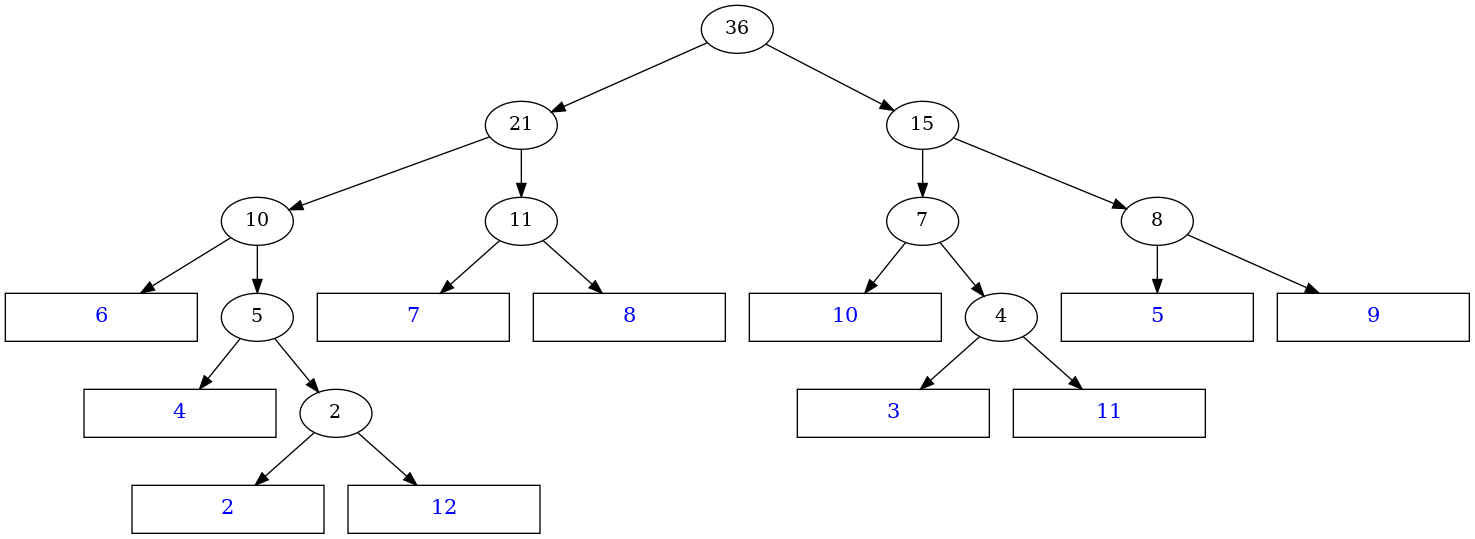
\includegraphics[width=\linewidth]{graphs/huffman_1.png}
	\caption{Huffman coding for $Z$}
	\label{fig:huffman_coding}
\end{figure}

The expected length of an encoding of $Z$ is then given as:
\begin{align*}
	E[\abs{C(Z)}] & = \sum_{z \in Z}{P(Z = z) \cdot \abs{C(Z)}} \\
	& = \frac{1}{36} (\abs{C(2)} + \abs{C(12)}) 
	+ \frac{2}{36} (\abs{C(3)} + \abs{C(11)}) 
	+ \frac{3}{36} (\abs{C(4)} + \abs{C(10)}) \\
	& + \frac{4}{36} (\abs{C(5)} + \abs{C(9)})
	+ \frac{5}{36} (\abs{C(6)} + \abs{C(8)})
	+ \frac{6}{36} (\abs{C(7)}) \\
	& = \frac{1}{36} (5 + 5)
	+ \frac{2}{36} (4 + 4)
	+ \frac{3}{36} (4 + 3) \\
	& + \frac{4}{36} (3 + 3)
	+ \frac{5}{36} (3 + 3)
	+ \frac{6}{36} (3) \\
	& \approx 3.31 \\
	& \leq H(Z) + 1
\end{align*}

\section{Codes}

Let $S$ be a random variable, with $P(S = s_1) = P(S = s_2) = 0.3$, $P(S = s_3)
= 0.2$, $P(S = s_4) = P(S = s_5) = 0.1$.

\subsection{Shannon coding $C_A$}

Let $p_i := P(S = s_i)$, $l_i := \ceil{-\log_2(p_i)}$. Let $(x)_2$ be the
binary expansion of $x$. A Shannon coding $C_A$ may be derived as shown in
table \ref{tbl:shannon_coding_1}.
\\

\begin{table}
	\centering
	\begin{tabu}{llllll}
		\toprule
		n & $p_i$ & $l_i$ & $\sum_{i = 0}^{n - 1}{p_i}$ & $(\sum_{i = 0}^{n - 1}{p_i})_2$ & $C_A(s_n)$ \\
		\midrule
		1 & 0.3 & 2 & $0$ & $0.00$ & $00$ \\
		2 & 0.3 & 2 & $0.3$ & $0.01\ldots$ & $01$ \\
		3 & 0.2 & 3 & $0.6$ & $0.100\ldots$ & $100$ \\
		4 & 0.1 & 4 & $0.8$ & $0.1100\ldots$ & $1100$ \\
		5 & 0.1 & 4 & $0.9$ & $0.1110\ldots$ & $1110$ \\
		\bottomrule
	\end{tabu}
	\caption{Shannon coding $C_A$}
	\label{tbl:shannon_coding_1}
\end{table}

Then:
\begin{align*}
	E[\abs{C_A(S)}] = 0.3 \cdot (2 + 2) + 0.2 \cdot 3 + 0.1 \cdot (4 + 4) = 2.6
\end{align*}

\subsection{Shorter code $C_B$}

As in the previous exercise we can derive a Huffman coding as shown in figure
\ref{fig:huffman_coding_2}.

\begin{figure}
	\centering
	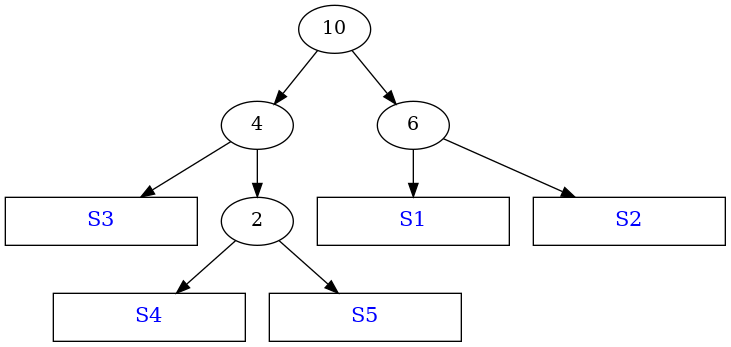
\includegraphics[width=\linewidth]{graphs/huffman_2.png}
	\caption{Huffman coding $C_B$}
	\label{fig:huffman_coding_2}
\end{figure}

Its average word length is given by:
\begin{align*}
	E[\abs{C_B(S)}] = 0.3 \cdot (2 + 2) + 0.2 \cdot 2 + 0.1 \cdot (3 + 3) = 2.2 < 2.6
\end{align*}

\subsection{$E[\abs{F_C(S_C)}] = H(S_C)$}

Let $S_C \sim Un(\{0, 1\})$. Let
\[
	F_C(s) :=
	\begin{cases}
		0, & \text{if } s = 0 \\
		1, & \text{if } s = 1
	\end{cases}
\]

Clearly $\abs{F_C(s)} = 1\ \forall\ s \in S_c \Rightarrow E[\abs{F_C(S_C)}] =
1$, and $H(S_C) = -(0.5 \log_2(0.5) + 0.5 \log_2(0.5)) = 1$.


\section{Perfect security}

\end{document}

